

\chapter{Regression and Reconstruction on \textit{d}-dimensional Cartesian Product Graphs}

\lhead{Chapter 6. \emph{Regression and Reconstruction on \textit{d}-dimensional Product Graphs}}

\label{chap:nd_gsp}

Multiway Graph Signal Processing (MWGSP) is an emerging field of research that seeks to generalise existing GSP algorithms, designed for use on graphs of one or two dimensions, to an arbitrary number of dimensions \citep{Stanley2020}. This introduces the concept 

The roles of tensors and is long-established in the 

\begin{figure}[t]
    \begin{center}
        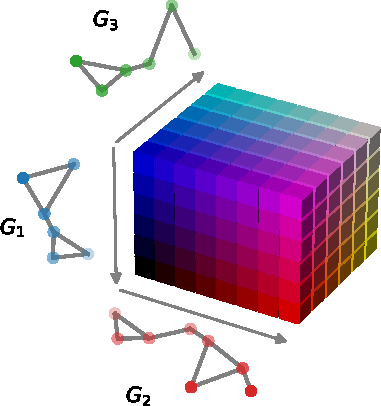
\includegraphics[width=0.4\linewidth]{Figures/coloured_tensor.pdf}
    \end{center}
    \caption[Graphical depiction of an order-3 tensor]{Graphical depiction of an order-3 tensor with graphs underlying each axis}
    \label{fig:3D_colored_tensor}
\end{figure}


In this chapter we extend the methods developed in the previous two chapters, that is Graph Signal Reconstruction (GSR), Kernel Graph Regression (KGR) and Regression with Network Cohesion (RNC), to graphs which are the Cartesian product of three or more factor graphs. 

\begin{itemize}
    \item Summarise chapter aims and output
\end{itemize}




\section{Extending GSP to arbitrary dimensions}

\subsection{The Cartesian product of more than two graphs}

In \cref{sec:graph_products_defined} we gave the general definition of a product between two graphs and highlighted four standard examples, namely the Cartesian, direct, strong and lexicographic products. Each of these product types can be straightforwardly extended to more than two factor graphs by applying their respective definition recursively. For example, consider the Cartesian product between graphs $\mathcal{G}_A = \{\mathcal{V}_A, \mathcal{E}_A\}$, $\mathcal{G}_B = \{\mathcal{V}_B, \mathcal{E}_B\}$ and $\mathcal{G}_C = \{\mathcal{V}_C, \mathcal{E}_C\}$ where $|\mathcal{V}_A| = A$, $|\mathcal{V}_B| = B$ and $|\mathcal{V}_C| = C$. This can be written as 

\begin{equation}
    \mathcal{G} \; = \; \mathcal{G}_A \, \square \; \mathcal{G}_B \, \square \; \mathcal{G}_C \; = \; \{\mathcal{V}, \, \mathcal{E}\}
\end{equation}

The new vertex set, $\mathcal{V}$, is given by the Cartesian product of the individual vertex sets. 

\begin{equation}
    \mathcal{V} = \mathcal{V}_A \times \mathcal{V}_B \times \mathcal{V}_C = \{(a, \, b, \, c) \in \mathbb{N}^3 \, | \, a \leq A, \; b \leq B, \text{and} \;  c \leq C\}
\end{equation}

The new edge set, $\mathcal{E}$, is given by recursively applying conditions 1 and 7 from, \cref{sec:graph_products_defined} to the new node set. In particular, any two nodes $(a, \, b, \, c)$ and $(a', b', c')$ are connected in $\mathcal{E}$ if they satisfy any of the following three conditions. 

\vspace{0.5cm}

\begin{table}[h]
    \def\arraystretch{1.5}
    \centering
    \begin{tabular}{lclclc}
        1. & $[a, \, a'] \in \mathcal{E}_A$    & and & $b = b'$  & and & $c = c'$             \\
        2. & $a = a'$    & and & $[b, \, b'] \in \mathcal{E}_B$   & and & $c = c'$             \\
        3. & $a = a'$    & and & $b = b'$  & and & $[c, \, c'] \in \mathcal{E}_C$              \\
    \end{tabular}
\end{table}


\begin{figure}[t]
    \begin{center}
        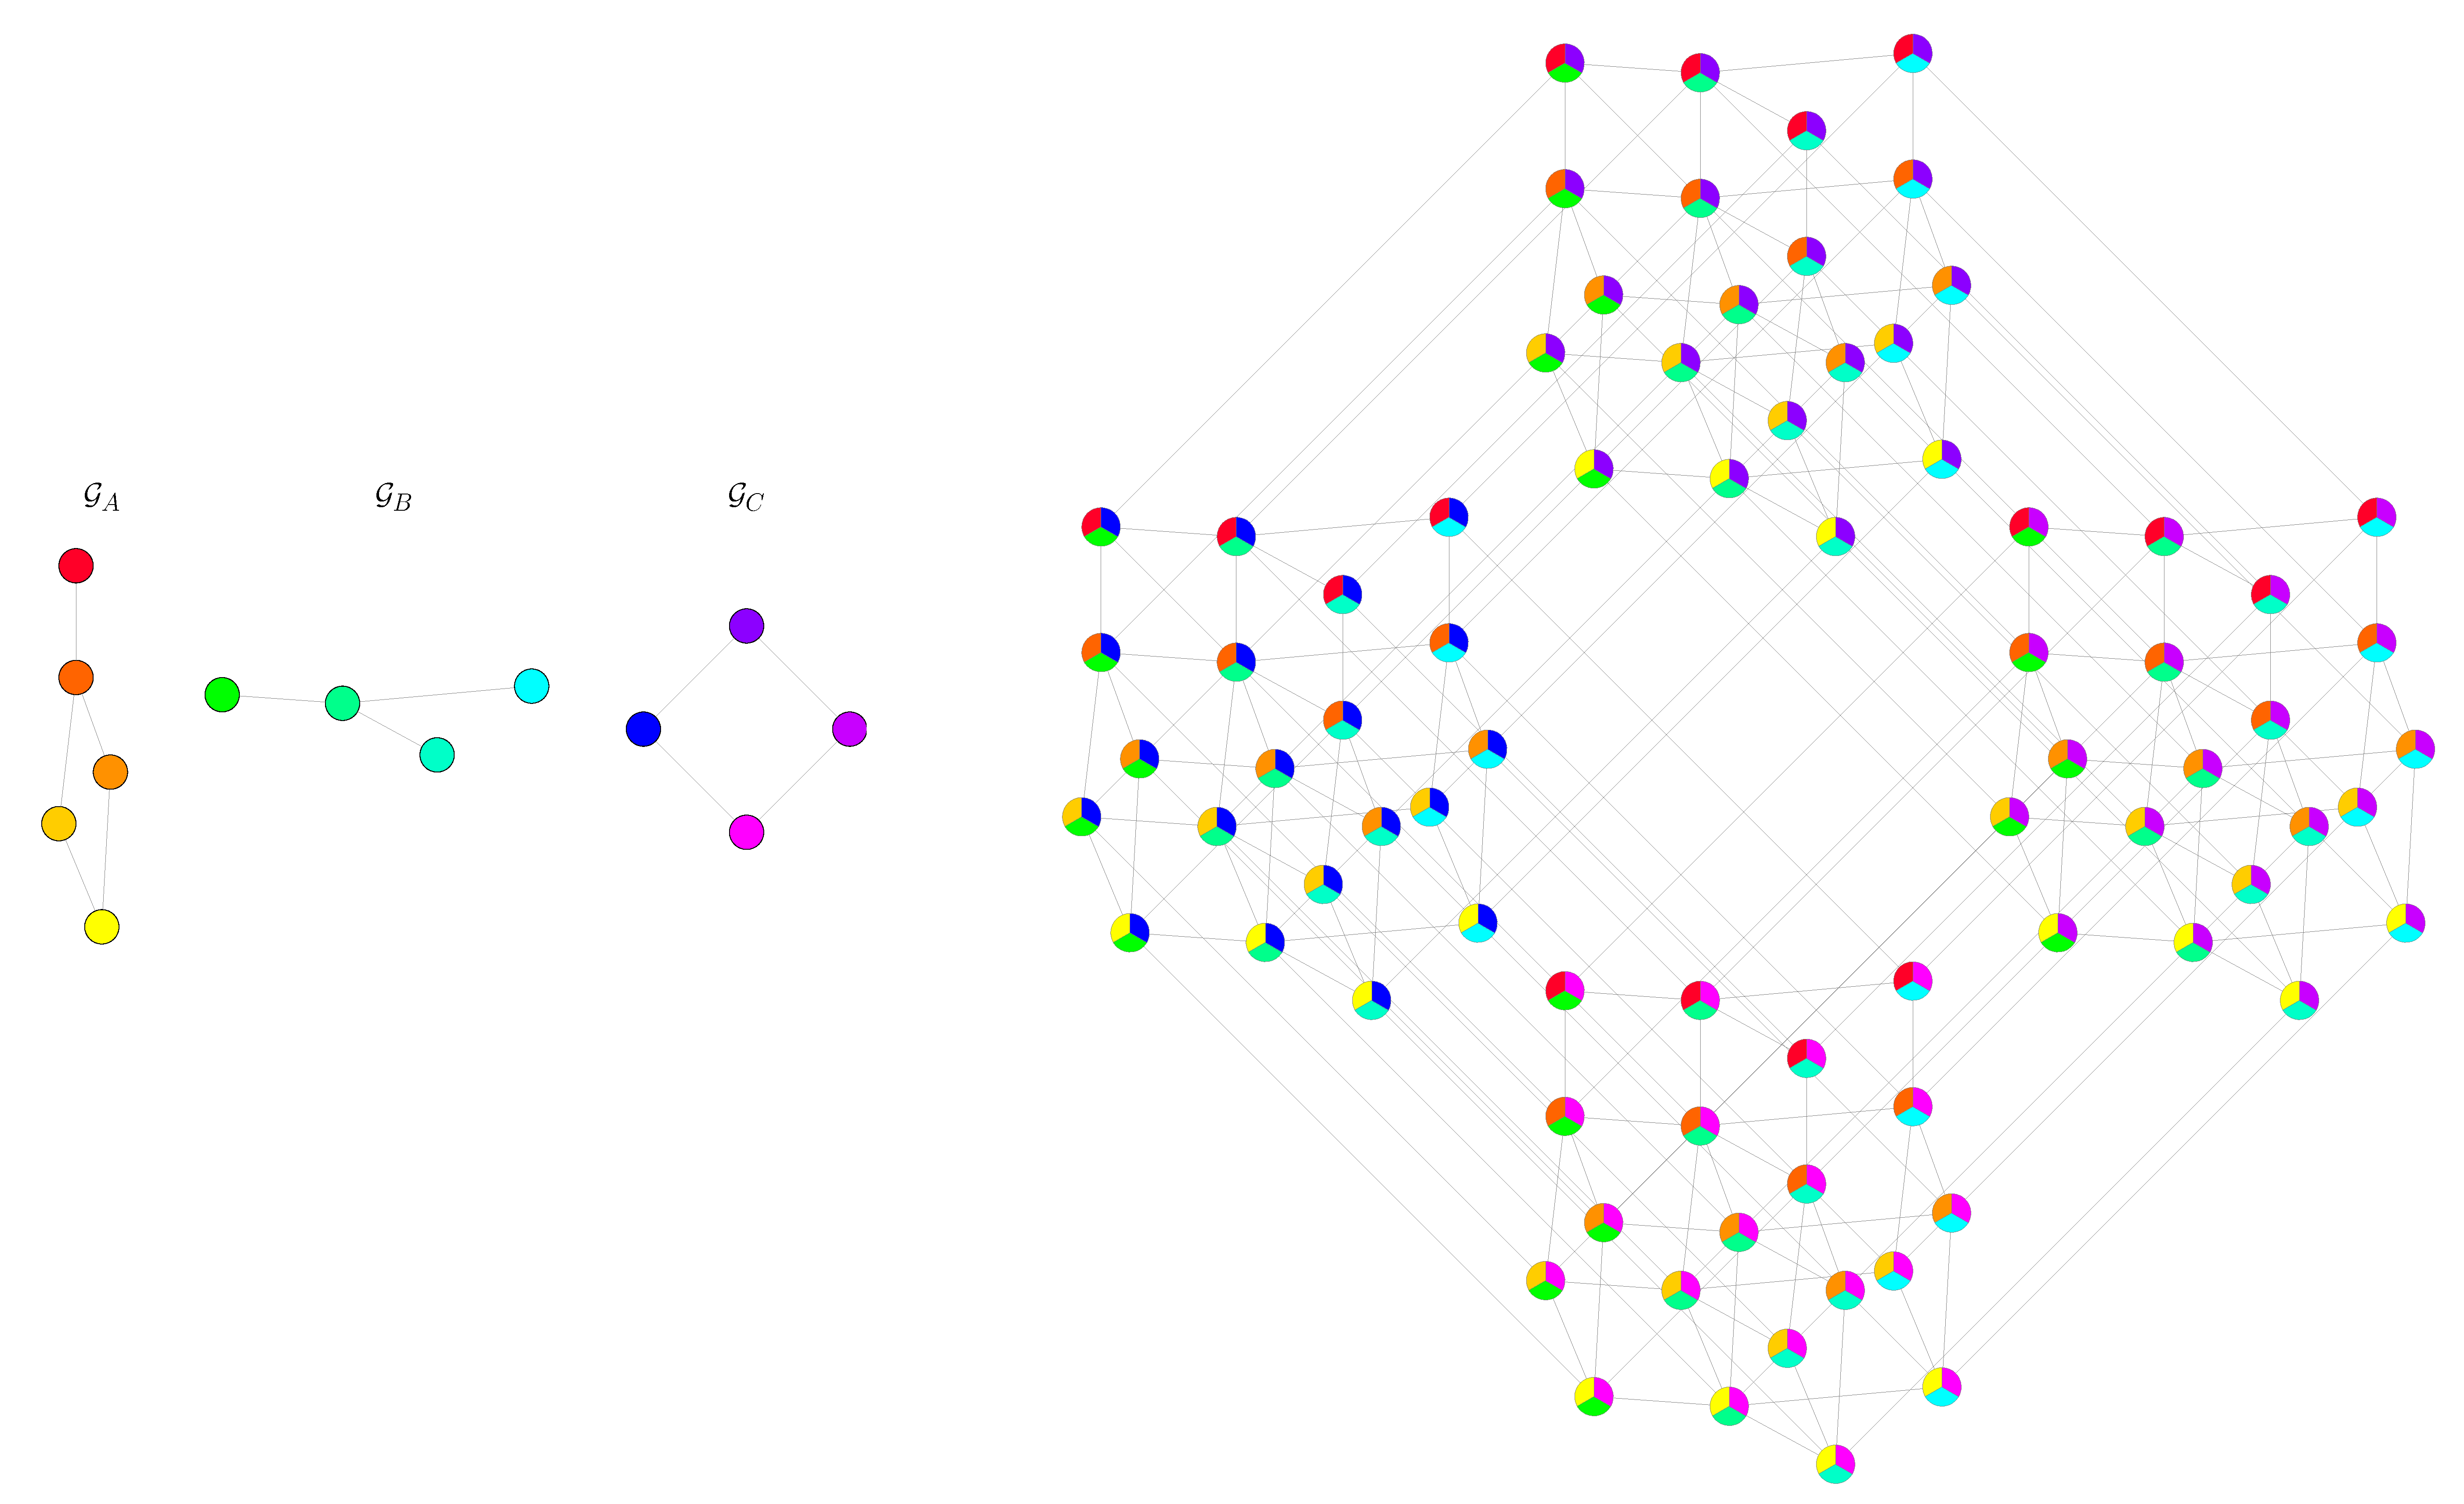
\includegraphics[width=\linewidth]{Figures/3D_CPG.pdf}
    \end{center}
    \caption[Graphical depiction of a 3D Cartesian product graph]{Graphical depiction of a 3D Cartesian product graph}
    \label{fig:3D_CPG}
\end{figure}

\Cref{fig:3D_CPG} gives a visual representation of a Cartesian product graph formed from three simple factor graphs. Notice that the size of the new vertex and edge set both grow very quickly. In particular, 

$$
|\mathcal{V}| = |\mathcal{V}_A| |\mathcal{V}_B| |\mathcal{V}_C| \aand |\mathcal{E}| =  |\mathcal{E}_A| |\mathcal{V}_B| |\mathcal{V}_C| + |\mathcal{V}_A| |\mathcal{E}_B| |\mathcal{V}_C| + |\mathcal{V}_A| |\mathcal{V}_B| |\mathcal{E}_C|
$$

Happily, the adjacency matrix of a Cartesian product graph $\A$ has a straightforward representation in terms of the factor adjacency matrices (here $\A_A$, $\A_B$ and $\A_C$). Specifically, it is given by the Kronecker sum

\begin{align}
    \A &= \A_A \oplus \A_B \oplus \A_C \notag \\
    &= \A_A \otimes \I_B \otimes \I_C  + \I_A \otimes \A_B \otimes \I_C + \I_A \otimes \I_B \otimes \A_C
\end{align}

In general, we can consider the Cartesian product of $d$ factor graphs with adjacency matrices denoted as $\A^{(1)} \in \R^{N_1 \times N_2}, \A^{(2)} \in \R^{N_2 \times N_2}, \dots \A^{(d)} \in \R^{N_d \times N_d}$. The full adjacency matrix will have size $N \times N$, where $N = \prod N_i$, and is given by  

\begin{alignat}{4}
    \A = \A^{(1)} & \oplus \A^{(2)} & \oplus \;\; ... \;\; & \oplus \A^{(d)} \notag \\[0.1cm]
    = \A^{(1)} & \otimes \I_{N_2} & \otimes \;\; ... \;\; & \otimes \I_{N_d} +  \notag \\[0.1cm]
    \I_{N_1} & \otimes \A^{(2)} & \otimes \;\; ... \;\; & \otimes \I_{N_d} + \;\; \ldots \;\; +  \notag \\[0.1cm]
    \I_{N_1} & \otimes \I_{N_2} & \otimes \;\; ... \;\; & \otimes \A^{(d)}  
\end{alignat}
    
This can be written compactly as 

\begin{equation}
    \A = \bigoplus_{i=1}^d  \A^{(i)}
\end{equation}

Similarly, the Laplacian of the product graph, $\LL$, can be written as the Kronecker sum of the individual factor graph Laplacians $\LL^{(i)}$. 

\begin{equation}
    \LL = \bigoplus_{i=1}^d  \LL^{(i)}
\end{equation}

We can perform eigendecomposition on each of the individual graph Laplacians as follows. 

\begin{equation}
    \LL^{(i)} = \U^{\,(i)} \LAM^{(i)} (\U^{\,(i)})^\top
\end{equation}

\noindent where $ \U^{(i)}$ is an orthogonal matrix such that each column is an eigenvector of $\LL^{(i)}$, and $\LAM^{(i)}$ is a diagonal matrix containing the corresponding eigenvalues, which are typically listed in ascending order. 

$$
\LAM^{(i)} = 
\begin{bmatrix}
    \lambda_1^{(i)}, &                 &        &                 \\
                     & \lambda_2^{(i)} &        &                 \\
                     &                 & \ddots &                 \\
                     &                 &        & \lambda_{N_i}^{(i)} \\
\end{bmatrix}
$$

Given this, the Laplacian of the product graph can be decomposed as follows. 

\begin{align}
    \LL &= \bigoplus_{i=1}^d \U^{\,(i)} \LAM^{(i)} (\U^{\,(i)})^\top \notag \\[0.2cm]
    &= \left( \bigotimes_{i=1}^d  \U^{\,(i)} \right) \left(\bigoplus_{i=1}^d \LAM^{(i)} \right) \left(\bigotimes_{i=1}^d  \U^{\,(i)} \right)^\top \notag \\[0.2cm]
    &= \U \LAM \U^\top 
\end{align}

\noindent where 

\begin{equation}
    \label{eq:U_LAM_def}
    \U =  \bigotimes_{i=1}^d  \U^{\,(i)} , \quad \text{and} \quad \LAM =  \bigoplus_{i=1}^d \LAM^{(i)}
\end{equation}


Here, we have used the notation $\bigotimes_{i=1}^d  \U^{\,(i)}$ to denote the chained Kronecker product of matrices $\{\U^{\,(i)}  \}$. 

\subsection{\textit{d}-dimensional graph signals}

A signal $\mathbfcal{Y}$ residing on the nodes of a $d$-dimensional product graph has a natural representation as a tensor of order $d$. One way to conceptualise a $d$-dimensional tensor signal is as a multi-dimensional array with $d$ independent axes. If the $i$-th factor graph has $N_i$ vertices, then $\mathbfcal{Y}$ will be of shape $(N_1 \times N_2 \times ... \times N_d)$. An individual element of this tensor signal can be specified via a vector index $\mathbf{n} = [n_1,\, n_2,\, ...,\, n_d]$, where $1\leq n_i \leq N_i$.

Alternatively, signals can be represented as a vector of length $N = \prod N_i$. This is essential if we are to interpret the $\otimes$ symbol strictly as a Kronecker product, rather than a tensor or outer product. Under the Kronecker interpretation, the chained use of $\otimes$ used in expressions such as \cref{eq:U_LAM_def} results in matrices of shape $N \times N$, providing a linear map from $\R^{N} \rightarrow \R^{N}$. Therefore, for an operator to act on a tensor graph signal $\mathbfcal{Y} \in \R^{N_1 \times N_2 \times ... \times N_d}$, we need a method of mapping tensors with shape $(N_1 \times N_2 \times ... \times N_d)$ to vectors of length $N$. In order for this vectorisation process to be consistent with the operators, it should result in a vectors whose elements are arranged in lexicographic order. In some fields, this is referred to as \textit{row-major} vectorisation since, in the case of an order-2 tensor, the index representing the row varies before the column index. In the following, we symbolise this operation mathematically as $\vecrm{\cdot}: \R^{N_1 \times N_2 \times ... \times N_d} \rightarrow \R^N$, and its reverse operation as $\text{ten}_\text{RM}\left(\cdot; \, (N_1, N_2, ..., N_d)\right): \R^N \rightarrow \R^{N_1 \times N_2 \times ... \times N_d}$. Note that the $text{ten}_\text{RM}$ function requires the expected output shape whereas $\vecrm{\cdot}$ does not. 

\begin{align*}
    \y \in \R^{N} = \vecrm{\mathbfcal{Y}}, \quad \implies \quad \mathbfcal{Y} \in \R^{N_1 \times N_2 \times ... \times N_d} =\text{ten}_\text{RM}\left(\y; \, (N_1, N_2, ..., N_d)\right)
\end{align*}

\Cref{fig:ten_to_vec} shows gives a visual summary of the for an order-3 tensor. 


\begin{figure}[t]
    \begin{center}
        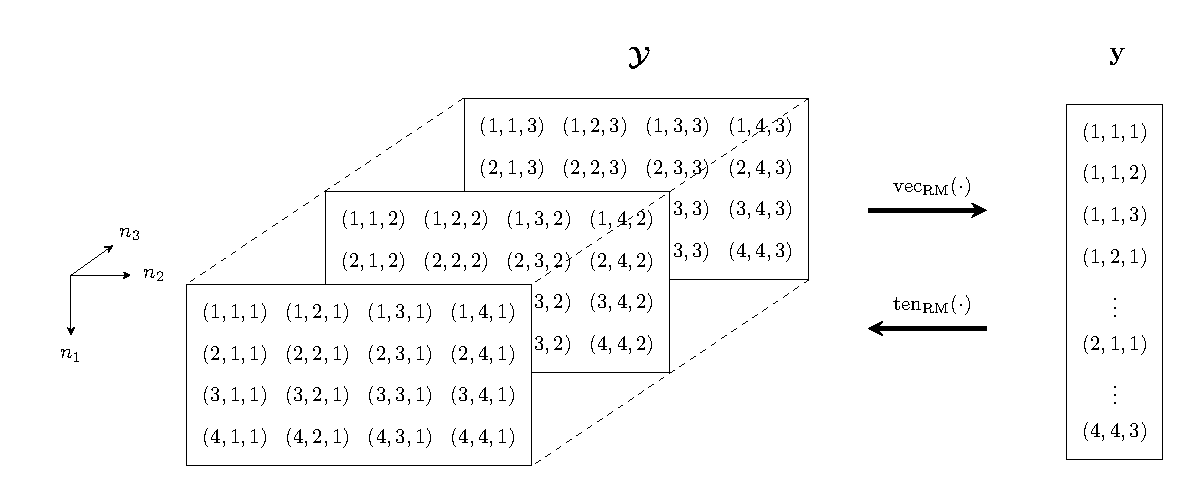
\includegraphics[width=\linewidth]{Figures/Tensor_Digaram.pdf}    
    \end{center}
    \caption{Graphical depiction of the process of converting an order-3 tensor between its multidimensional array and vectorised forma in row-major order. Note that the elements in the vectorised signal are lexicographically ordered. }
    \label{fig:ten_to_vec}
\end{figure}


\note{A note on tensor notation}{
    The use of tensor algebra is well established in fields such as phyics and mechanics \citep{Renteln2013,Abraham1988}, however, it is less commonly found in the signal processing community. For this reason, we choose to adopt a notation that leans more on linear algebra. In the process there is some loss of elegance, however, it has the benefit of fewer floating indices to keep track of. This is especially helpful when operating in a variable number of dimensions $d$. In general, all the equations and algorithms discussed in the following chapters could be alternatively written in tensor notation. For example, consider the following operation where a tensor $\mathbfcal{Z}$ is vectorised in row major order, then mapped by a matrix that is the chained Kronecker product of $d$ square matrices, and then turned back into a tensor in row major order. In our notation, this is written as

    \begin{equation}
        \label{eq:LA_MM}
        \mathbfcal{Y} = \text{ten}_{\text{RM}}\left(\left(\bigotimes_{i=1}^d  \U^{\,(i)}\right) \text{vec}_\text{RM}\left(\mathbfcal{Z}\right) \right)    
    \end{equation}

    In much of the following, we assume tensors exist in their vectorised form, meaning this can be reduced to 

    \begin{equation}
    \label{eq:LA_MM2}
    \y = \U \z, \where \U = \bigotimes_{i=1}^d  \U^{\,(i)}
    \end{equation}

    In more classical tensor notation, using the Einstein summation convention, \cref{eq:LA_MM} could be written as 

    \begin{equation}
    \label{eq:TEN_MM}
    \mathbfcal{Y}^{i_1, i_2, ..., i_d} = \left(\U^{(1)}\right)^{i_1}_{j_1}\left(\U^{(2)}\right)^{i_2}_{j_2} ... \left(\U^{(d)}\right)^{i_d}_{j_d} \, \mathbfcal{Z}^{j_1, j_2, ..., j_d}
    \end{equation}

    Note that here the indices $j_1, j_2, ..., j_d$, which as contravariant in $\z$ and covariant in $\U$, are implicitly summed over. This eliminates the need to consider vectorisation at all. Both forms offer different trade-offs, however, there is little practical difference when it comes to executing the signal precessing algorithms themselves as the full $N \times N$ matrix implied by \cref{eq:LA_MM,eq:LA_MM2} is never actually instantiated in memory. 

}

To calculate the vector index $k$ which a tensor element with index $\mathbf{n} = [n_1,\, n_2,\, ...,\, n_d]$ is mapped to in row-major order, we can apply the following formula.  

\begin{equation}
    \label{eq:vec}
    k = 1 + \sum_{i=1}^d \Big( \prod_{j=i+1}^d N_j \Big) \, (n_i - 1)
\end{equation}

(Note the $\pm1$ disappear when indexing begins from zero). The reverse operation, i.e. mapping a vector element index $k$ to a tensor index $\mathbf{n}$ can be achieved by running the algorithm \hyperlink{vectoten}{\textbf{3}}. 


\begin{algorithm}[t]
    \hypertarget{vectoten}{}
    \label{al:vectoten}
    \caption{Mapping a vector element to a tensor element in row major order}
    \begin{algorithmic}
    \vspace{0.15cm}
    \Require{The target vector element $k$} 
    \vspace{0.1cm}
    \Require{The shape of the output tensor $(N_1, N_2, ..., N_d)$} 
    \vspace{0.25cm}
    \State{$k \leftarrow  k - 1$}
    \vspace{0.25cm}
    \For{$i$ \textbf{from} $d$ \textbf{to} 1}
    \vspace{0.25cm}
    \State{$n_i \leftarrow  k \mod N_i$}
    \vspace{0.15cm}
    \State{$k \leftarrow \lfloor k / N_i \rfloor$} 
    \vspace{0.15cm}
    \EndFor
    \vspace{0.25cm}
    \Ensure{$(n_1 + 1, n_2 + 1, ..., n_d + 1)$}
    \end{algorithmic}
    \end{algorithm}



Given these two operations, two arrays of any consistent shape can be mapped between one another by first vectorising according to \cref{eq:vec}, and then converting to a tensor using the given algorithm.



\subsection{\textit{d}-dimensional graph signal processing}



Consider a graph signal $\y \in \R^N$ represented in its vectorised form. We can define the Graph Fourier Transform (GFT) and the corresponding inverse (IGFT) of this signal as follows. 

\begin{alignat}{2}
\label{eq:gft_nd}
    \text{GFT}(\y) & = \U^\top \y && = \Big(  \bigotimes_{i=1}^d  \U^{\,(i)} \Big)^\top \y \\
\label{eq:igft_nd}
    \text{IGFT}(\y) & = \U \y && = \Big(  \bigotimes_{i=1}^d  \U^{\,(i)} \Big) \; \y 
\end{alignat}

The concept of a graph filter for signals defined on a Cartesian product graph follows naturally from this definition. Just as in the one and two-dimensional case, a graph filter is constructed by first taking the GFT of a signal, then applying some scaling function to each spectral component, then transforming back into the vertex domain via the IGFT. In the simplest case, we can consider an isotropic graph filter function $g(\lambda, \beta)$, such as one of those defined in \cref{tab:iso_filters}. 


\begin{align}
    \HH &= \left( \bigotimes_{i=1}^d  \U^{\,(i)} \right) g\left(\bigoplus_{i=1}^d \LAM^{(i)}; \beta \right) \left(\bigotimes_{i=1}^d  \U^{\,(i)} \right)^\top \notag \\[0.2cm]
        &= \U \, \Diag{\vecrm{\mathbfcal{G}}} \, \U^\top
\end{align}


Here, $\mathbfcal{G}$ represents the spectral scaling tensor, which has element $\mathbf{n} = [n_1,\, n_2,\, ...,\, n_d]$ given by 

\begin{equation}
    \mathbfcal{G}_{\mathbf{n}} = g\left(\sum_{i=1}^d \lambda^{(i)}_{n_i}; \, \beta\right)
\end{equation}

This can be further generalised to a anisotropic graph filter function, where the intensity of the filtering operation is not restricted to be equal in each dimension. \Cref{tab:anis_filters} gives some examples of anisotropic graph filter functions defined to act in an arbitrary number of dimensions. Notice how the definition of  

\begin{table}[t]
    \def\arraystretch{1.7}
    \small
    \begin{center}
        \begin{tabular}{|l|c|}
            \hline
            \textbf{Filter}   & $g(\lambdaa; \,\betaa)$                                            \\
            \hline
            1-hop random walk & $(1 + \betaa^\top\lambdaa)^{-1}$                                   \\
            \hline
            Diffusion         & $\exp(-\betaa^\top\lambdaa)$                                       \\
            \hline
            ReLu              & $\max (1 - \betaa^\top\lambdaa, 0)$                                \\
            \hline
            Sigmoid           & $2 \big( 1 + \exp(\betaa^\top\lambdaa)\big)^{-1}$                  \\
            \hline
            Bandlimited       & $1, \,\text{if} \; \betaa^\top\lambdaa \leq 1 \; \text{else} \; 0$ \\
            \hline
        \end{tabular}
    \end{center}
    \caption{Anisotropic graph filter functions in an arbitrary number of dimensions}
    \label{tab:anis_filters}
\end{table}


In this case, the spectral scaling tensor is given by 

\begin{equation}
    \mathbfcal{G}_{\mathbf{n}} = g\big(\lambdaa(\mathbf{n}); \, \betaa\big)
\end{equation}

where $\betaa \in \R^{d}$ is the parameter vector characterising the filter intensity in each dimension, and $\lambdaa(\mathbf{n}) \in \R^d$ is a vector holding the $n_i$-th eigenvalue of each graph Laplacian in the Cartesian product. 

$$
\lambdaa(\mathbf{n}) = 
\begin{bmatrix}
    \lambda^{(1)}_{n_1} & \lambda^{(2)}_{n_2} & \dots & \lambda^{(d)}_{n_d}    
\end{bmatrix}^\top
$$

\subsection{Fast computation with \textit{d}-dimensional Kronecker products}

Consider the graph Fourier and inverse Fourier transforms of a $d$-dimensional graph signal given in \cref{eq:gft_nd,eq:igft_nd}. In both cases, we are required to compute the result of a chained Kronecker product matrix acting on a length-$N$ vector. Whilst the obvious approach to computing this product would have time and memory complexity of $O(N^2)$, a much more efficient implementation can be achieved by taking advantage of the Kronecker structure of the matrix. In practice, the required memory and time complexity can be reduced to $O(N)$ and $O(N\sum N_i)$ respectively. 

This algorithm for achieving this is well-known, and can be summarised as follows. Consider the application of a chained Kronecker product matrix acting on a vector $\y$. 

$$
\x = \left( \C^{(1)} \otimes \C^{(2)} \otimes ... \otimes \C^{(d)}\right) \y
$$

This can be factorised as follows

$$
\x = \left( \C^{(1)} \otimes \I \otimes ... \otimes \I \right)\left( \I \otimes \C^{(2)} \otimes ... \otimes \I \right) ... \left( \I \otimes \I \otimes ... \otimes \C^{(d)} \right) \y
$$

As is visible, the original multiplication has now been broken into $d$ stages. However, the $i$-th matrix-vector multiplication can be completed in $O(N_i N)$ operations by reshaping the vector in the appropriate way and leveraging the properties of the Kronecker product. The reshaping operation can be completed using strided permutation matrices which can be applied in practice for virtually zero computational cost \citep{Granata1992}. This idea is also key to the FFT and related algorithms, which can be understood as finding a recursive Kronecker structure in the Fourier matrix \citep{Tolimieri2013}. 

Work on efficient computational procedures for this operation can be traced back to \cite{Roth1934} who proposed the original 2-dimensional ``vec trick" algorithm. The $d$-dimensional algorithm was obtained in \cite{Pereyra1973} and improved in \cite{DeBoor1979}. More recent work, such as \cite{Fackler2019}, has focused on further optimisations such as minimising data transit times and parallel processing. 

In order to execute computations of this nature in a way that is maximally efficient, we have developed the Python library \textit{PyKronecker}, which is described in detail in \cite{Antonian2023}. This library offers a high-level API for constructing Kronecker-based operators and applying them to either vectors or tensors, whilst optimising the underlying computation using parallel GPU processing and Just In Time (JIT) compilation. 


\begin{algorithm}[t]
\hypertarget{alkronx}{}
\label{al:kronx}
\caption{The \text{kronx} method}
\begin{algorithmic}
\vspace{0.15cm}
\Require{List of square matrices $\{\M^{(i)} \in \R^{N_{i} \times N_{i}}\}_{i=1}^d$} 
\vspace{0.1cm}
\Require{$d$-dimensional tensor $\mathbfcal{Y} \in \R^{N_1 \times N_2 \times \; ... \; \times N_d}$} 
\vspace{0.25cm}
\State{$\Y \leftarrow \text{reshape}\Big(\mathbfcal{Y}, \; \big(N_1,\, \frac{N}{N_1}\big) \Big)$}
\vspace{0.25cm}
\For{$i$ \textbf{from} 1 \textbf{to} $d$}
\vspace{0.25cm}
\State{$\Y \leftarrow \text{reshape}\Big(\Y, \big(N_i  \times \frac{N}{N_i}\big) \Big)$}
\vspace{0.15cm}
\State{$\Y \leftarrow \big( \M^{(i)} \; \Y  \big)^\top$} 
\vspace{0.15cm}
\EndFor
\vspace{0.25cm}
\Ensure{$\text{reshape}\Big(\Y, \big(N_1 \times N_2 \times \; ... \; \times N_d \big) \Big)$}
\end{algorithmic}
\end{algorithm}

\section{Tensor Graph Signal reconstruction}

The model we use to describe graph signal reconstruction in the multi-dimensional setting is as follows. Consider a tensor signal $\mathbfcal{Y}$ of shape $\big(N_1 \times N_2 \times \; ... \; \times N_d \big)$ with elements interpreted as existing on the nodes of a $d$-dimensional Cartesian product graph. Only a partial set $\mathcal{S}$ of the elements of $\mathbfcal{Y}$ are available at observation time, with unobserved values set to zero. The goal is to estimate the signal value at these unobserved entries. 

The binary sensing tensor $\mathbfcal{S}$, of the same shape as $\mathbfcal{Y}$, indicates which elements of $\mathbfcal{Y}$ were observed in the following way 

\begin{equation}
    \mathbfcal{S}_{n_1,n_2,...n_d} = \begin{cases}
        1 & \text{if} \;\; (n_1,n_2,...n_d) \in \mathcal{S} \\
        0 & \text{otherwise}
    \end{cases}
\end{equation}

In analogy with the two dimensional case, (see \cref{sec:problem_statement_2d}), we assume that $\mathbfcal{Y}$ is a noisy partial observation of an underlying tensor $\mathbfcal{F}$ which is smooth with respect to the topology of the Cartesian product graph. This is represented in the following statistical model. 

\begin{equation}
    \mathbfcal{Y} = \mathbfcal{S} \circ \big(\mathbfcal{F} + \mathbfcal{E} \big)
\end{equation}

where, here, the $\circ$ symbol represents the generalised tensor Hadamard product, i.e. element-wise multiplication of two tensors. $\mathbfcal{E}$ is a random tensor where each element has an independent normal distribution with with unit variance. That is,

\begin{equation}
    \vecrm{\mathbfcal{E}} = \sim \mathcal{N}(\mathbf{0}, \, \I)
\end{equation}

Given this error distribution, the conditional distribution of $\mathbfcal{Y} |  \mathbfcal{F}$ is given by 

\begin{equation}
    \vecrm{\mathbfcal{Y}} \, | \, \vecrm{\mathbfcal{F}} \, \sim \, \mathcal{N}\Big(\vecrm{\mathbfcal{S} \circ \mathbfcal{F}}, \; \Diag{\vecrm{\mathbfcal{S}}}\Big)
\end{equation}

Or, more concisely, 

\begin{equation}
    \y \, | \, \f \, \sim \, \mathcal{N}\big(\s \circ \f, \; \diag{\s}\big)
\end{equation}


\section{Kernel Graph Tensor Regression}

Hello

\section{Tensor Regression with Network Cohesion}

Ahhhh

